\subsection{Quadratic forms}

One of the applications of orthogonal diagonalization is that of quadratic forms and graphs of level curves of a quadratic form. This section has to do with rotation of axes
so that with respect to the new axes, the graph of the level curve of a
quadratic form is oriented parallel to the coordinate axes. This makes it
much easier to understand. For example, we all know that $x_1^2 + x_2^2=1$ represents the equation in two variables whose graph in $\mathbb{R}^2$ is a circle of radius $1$. But how do we know what the graph of the equation $5x_1^2 + 4x_1x_2 + 3x_2^2=1$ represents?  
\index{principal axis!quadratic forms}

We first formally define what is meant by a quadratic form. In this section we will work with only \textit{real} quadratic forms, which means that the coefficients will all be real numbers. 

\begin{definition}{Quadratic form}{quadraticform}
A \textbf{quadratic form}\index{quadratic form} is a polynomial of degree two in $n$ variables $x_1, x_2, \cdots, x_n$, written as a linear combination of $x_i^{2}$ terms and $x_ix_j$ terms. 
\end{definition}

Consider the quadratic form $q = a_{11}x_1^2 + a_{22}x_2^2 + \cdots + a_{nn}x_n^2 + a_{12}x_1x_2 + \cdots$. We can write $\vect{x} = \leftB 
\begin{array}{r}
x_1 \\
x_2 \\
\vdots \\
x_n
\end{array} \rightB$ as the vector whose entries are the variables contained in the quadratic form.

Similarly, let $A = \leftB
\begin{array}{rrrr}
a_{11} & a_{12} & \cdots & a_{1n} \\
a_{21} & a_{22} & \cdots & a_{2n} \\
\vdots & \vdots & & \vdots \\
a_{n1} & a_{n2} & \cdots & a_{nn}
\end{array}
\rightB$ be the matrix whose entries are the coefficients of $x_i^2$ and $x_ix_j$ from $q$. Note that the matrix $A$ is not unique, and we will consider this further in the example below. Using this matrix $A$,  the quadratic form can be written as $q = \vect{x}^T A \vect{x}$. 

\begin{eqnarray*}
q &=& \vect{x}^T A \vect{x} \\
&=& \leftB \begin{array}{rrrr}
x_1 & x_2 & \cdots & x_n
\end{array} \rightB 
 \leftB
\begin{array}{rrrr}
a_{11} & a_{12} & \cdots & a_{1n} \\
a_{21} & a_{22} & \cdots & a_{2n} \\
\vdots & \vdots & & \vdots \\
a_{n1} & a_{n2} & \cdots & a_{nn}
\end{array}
\rightB
\leftB \begin{array}{r}
x_1 \\
x_2 \\
\vdots \\
x_n 
\end{array}
\rightB \\
&=& 
\leftB \begin{array}{rrrr}
x_1 & x_2 & \cdots & x_n
\end{array} \rightB 
\leftB
\begin{array}{c}
a_{11}x_1 + a_{21}x_2 + \cdots + a_{n1}x_n \\
a_{12}x_1 + a_{22}x_2 + \cdots + a_{n2}x_n \\
\vdots \\
a_{1n}x_1 + a_{2n}x_2 + \cdots + a_{nn}x_n
\end{array}
\rightB \\
&=& a_{11}x_1^2 + a_{22}x_2^2 + \cdots + a_{nn}x_n^2 + a_{12}x_1x_2 + \cdots
\end{eqnarray*}

Let's explore how to find this matrix $A$. Consider the following example.

\begin{example}{Matrix of a quadratic form}{matrixquadraticform}
Let a quadratic form $q$ be given by 
\[
q = 6x_1^2 + 4x_1x_2 + 3x_2^2
\]
Write $q$ in the form $\vect{x}^TA\vect{x}$. 
\end{example}

\begin{solution}
First, let $\vect{x} = \leftB
\begin{array}{r}
x_1 \\
x_2
\end{array}
\rightB$ and $A = \leftB
\begin{array}{rr}
a_{11} & a_{12} \\
a_{21} & a_{22}
\end{array}
\rightB$. 

Then, writing $q = \vect{x}^TA\vect{x}$ gives 
\begin{eqnarray*}
q &=& \leftB \begin{array}{rr}
x_1 & x_2 
\end{array}
\rightB
\leftB \begin{array}{rr}
a_{11} & a_{12} \\
a_{21} & a_{22}
\end{array}
\rightB
\leftB \begin{array}{r}
x_1 \\
x_2 
\end{array}
\rightB \\
&=& a_{11}x_1^2 + a_{21}x_1x_2 + a_{12}x_1x_2 + a_{22}x_2^2
\end{eqnarray*}

Notice that we have an $x_1x_2$ term as well as an $x_2x_1$ term. Since multiplication is commutative, these terms can be combined. This means that $q$ can be written 
\[
q =  a_{11}x_1^2 + \left( a_{21}+ a_{12}\right) x_1x_2 + a_{22}x_2^2
\]

Equating this to $q$ as given in the example, we have 
\[
 a_{11}x_1^2 + \left( a_{21}+ a_{12}\right) x_1x_2 + a_{22}x_2^2 =  6x_1^2 + 4x_1x_2 + 3x_2^2
\]

Therefore,
\begin{eqnarray*}
a_{11} &=& 6 \\
a_{22} &=& 3 \\
a_{21}+a_{12} &=& 4
\end{eqnarray*}

This demonstrates that the matrix $A$ is not unique, as there are several correct solutions to $a_{21}+a_{12} = 4$. However, we will \textit{always} choose the coefficients such that $a_{21} = a_{12} = \frac{1}{2} (a_{21}+a_{12})$. This results in $a_{21} = a_{12} = 2$. This choice is key, as it will ensure that $A$ turns out to be a symmetric matrix.  

Hence, 
\[
A = 
\leftB \begin{array}{rr}
a_{11} & a_{12} \\
a_{21} & a_{22}
\end{array}
\rightB
=
\leftB
\begin{array}{rr}
6 & 2 \\
2 & 3
\end{array}
\rightB
\]

You can verify that $q = \vect{x}^T A \vect{x}$ holds for this choice of $A$. 
\end{solution}

The above procedure for choosing $A$ to be symmetric applies for any quadratic form $q$. We will \textit{always} choose coefficients such that $a_{ij}=a_{ji}$. 

We now turn our attention to the focus of this section. Our goal is to start with a quadratic form $q$ as given above and find a way to rewrite it to eliminate the $x_ix_j$ terms. This is done through a change of variables. In other words, we wish to find $y_i$ such that 
\[
q = d_{11}y_1^2 + d_{22}y_2^2 + \cdots + d_{nn}y_n^2
\]
 Letting $\vect{y} = \leftB
\begin{array}{r}
y_1 \\
y_2 \\
\vdots \\
y_n
\end{array}
\rightB$ and $D = \leftB d_{ij} \rightB$, we can write $q = \vect{y}^T D \vect{y}$ where $D$ is the matrix of coefficients from $q$. There is something special about this matrix $D$ that is crucial. Since no $y_iy_j$ terms exist in $q$, it follows that $d_{ij} = 0$ for all $i \neq j$. Therefore, $D$ is a diagonal matrix. Through this change of variables, we find the \textbf{principal axes}\index{principal axes} $y_1, y_2, \cdots, y_n$ of the quadratic form. 

This discussion sets the stage for the following essential theorem.

\begin{theorem}{Diagonalizing a quadratic form}{diagquadraticform}
Let $q$ be a quadratic form in the variables $x_1, \cdots, x_n$. It follows that $q$ can be written in the form $q = \vect{x}^T A \vect{x}$ where 
\[
\vect{x} = \leftB \begin{array}{r}
x_1 \\
x_2 \\
\vdots \\
x_n
\end{array} \rightB 
\]
and $A = \leftB a_{ij} \rightB$ is the symmetric matrix of coefficients of $q$. 

New variables $y_1, y_2, \cdots, y_n$ can be found such that $q = \vect{y}^T D \vect{y}$ where 
\[
\vect{y} = \leftB \begin{array}{r} 
y_1 \\
y_2 \\
\vdots \\
y_n
\end{array} \rightB \] and $D=\leftB d_{ij} \rightB$ is a diagonal matrix. The matrix $D$ contains the eigenvalues of $A$ and is found by orthogonally diagonalizing $A$. 
\end{theorem}

While not a formal proof, the following discussion should convince you that the above theorem holds. Let $q$ be a quadratic form in the variables $x_1, \cdots, x_n$. Then, $q$ can be written in the form $q = \vect{x}^T A \vect{x}$ for a symmetric matrix $A$.  
By Theorem \ref{thm:orthdiag} we can orthogonally diagonalize the matrix $A$ such that $U^TAU = D$ for an orthogonal matrix $U$ and diagonal matrix $D$. 

Then, the vector $\vect{y} = \leftB \begin{array}{r}
y_1 \\
y_2 \\
\vdots \\
y_n
\end{array}
\rightB
$ is found by $\vect{y} = U^T \vect{x}$. To see that this works, rewrite $\vect{y} = U^T \vect{x}$ as $\vect{x} = U\vect{y}$. Letting $q = \vect{x}^TA\vect{x}$, proceed as follows:
\begin{eqnarray*}
q &=& \vect{x}^T A \vect{x}\\
&=& (U\vect{y})^T A (U\vect{y})\\
&=& \vect{y}^T (U^TAU) \vect{y} \\
&=& \vect{y}^T D \vect{y}
\end{eqnarray*}

The following procedure details the steps for the change of variables given in the above theorem. 

\begin{procedure}{Diagonalizing a quadratic form}{diagquadraticform}
Let $q$ be a quadratic form in the variables $x_1, \cdots, x_n$ given by 
\[
q = a_{11}x_1^2 + a_{22}x_2^2 + \cdots + a_{nn}x_n^2 + a_{12}x_1x_2+\cdots
\]
Then, $q$ can be written as $q = d_{11}y_1^2 + \cdots + d_{nn}y_n^2$ as follows:

\begin{enumerate}
\item
Write $q = \vect{x}^T A \vect{x}$ for a symmetric matrix $A$. 

\item
Orthogonally diagonalize $A$ to be written as $U^TAU=D$ for an orthogonal matrix $U$ and diagonal matrix $D$. 

\item
Write $\vect{y} = \leftB \begin{array}{c}
y_1 \\
y_2 \\
\vdots \\
y_n
\end{array}
\rightB$. Then, $\vect{x} = U \vect{y}$. 

\item 
The quadratic form $q$ will now be given by 
\[
q = d_{11}y_1^2 + \cdots + d_{nn}y_n^2 = \vect{y}^T D \vect{y}
\]
where $D = \leftB d_{ij} \rightB$ is the diagonal matrix found by orthogonally diagonalizing $A$. 
\end{enumerate}
\end{procedure}

Consider the following example. 

\begin{example}{Choosing new axes to simplify a quadratic form}{newaxes1}
Consider the following level curve
\[
6x_1^2 + 4x_1x_2 + 3x_2^2 = 7
\]
shown in the following graph. 
\begin{center}
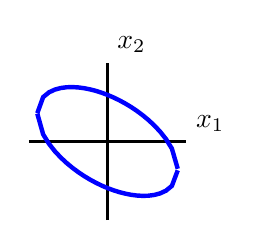
\begin{tikzpicture}[scale=0.5]
\draw[-, thick](-2,0)--(2,0);
\node[above right] at (2,0){$x_1$};
\draw[-, thick](0,-2)--(0,2);
\node[above right] at (0,2){$x_2$};
\draw[blue, ultra thick, domain=-1.78376:1.78376] plot(\x, {0.2*(-2*\x-sqrt(35-11*\x*\x))});
\draw[blue, ultra thick, domain=-1.78376:1.78376] plot(\x, {0.2*(sqrt(35-11*\x*\x)-2*\x)});
\end{tikzpicture}
\end{center}

Use a change of variables to choose new axes such that the ellipse is oriented parallel to the new coordinate axes. In other words, use a change of variables to rewrite $q$ to eliminate the $x_1x_2$ term. 
\end{example}

\begin{solution}
Notice that the level curve is given by $q = 7$ for $q = 6x_1^2 + 4x_1x_2 + 3x_2^2$. This is the same quadratic form that we examined earlier in Example \ref{exa:matrixquadraticform}. Therefore we know that we can write $q = \vect{x}^T A \vect{x}$ for the matrix 
\[
A = \leftB
\begin{array}{rr}
6 & 2 \\
2 & 3
\end{array}
\rightB
\]

Now we want to orthogonally diagonalize $A$ to write $U^TAU=D$ for an orthogonal matrix $U$ and diagonal matrix $D$. The details are left to the reader, and you can verify that the resulting matrices are 
\begin{eqnarray*}
U &=& 
\leftB
\begin{array}{rr}
\vspace{0.05in}\frac{2}{\sqrt{5}} & -\vspace{0.05in}\frac{1}{\sqrt{5}} \\
\vspace{0.05in}\frac{1}{\sqrt{5}} & \vspace{0.05in}\frac{2}{\sqrt{5}}
\end{array}
\rightB \\
D &=& 
\leftB
\begin{array}{rr}
 7 & 0 \\
0 & 2 
\end{array}
\rightB
\end{eqnarray*}

Next we write $ \vect{y} = \leftB 
\begin{array}{c}
y_1 \\
y_2 
\end{array}
\rightB$. It follows that $\vect{x} = U \vect{y}$. 

We can now express the quadratic form $q$ in terms of $y$, using the entries from $D$ as coefficients as follows:
\begin{eqnarray*}
q &=& d_{11}y_1^2 + d_{22}y_2^2 \\
&=& 7y_1^2 + 2y_2^2 
\end{eqnarray*}

Hence the level curve can be written $7y_1^2 + 2y_2^2 =7$. 
The graph of this equation is given by:

\begin{center}
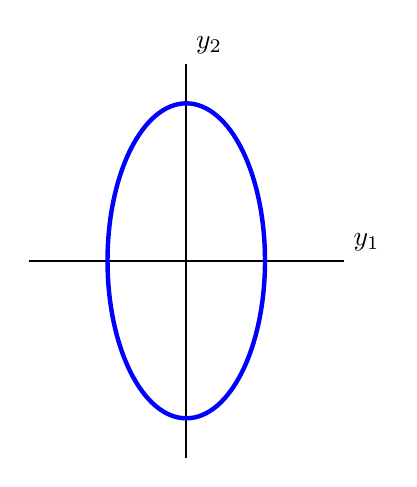
\begin{tikzpicture}
\draw[-, thick](-2,0)--(2,0);
\node[above right] at (2,0){$y_1$};
\draw[-, thick](0,-2.5)--(0,2.5);
\node[above right] at (0,2.5){$y_2$};
\draw[ultra thick, blue] (0,0) ellipse (1cm and 2cm);
\end{tikzpicture}
\end{center}

The change of variables results in new axes such that with respect to the new axes, the ellipse is oriented parallel to the coordinate axes. These are called the \textbf{principal axes} of the quadratic form. 
\end{solution}

The following is another example of diagonalizing a quadratic form. 

\begin{example}{Choosing new axes to simplify a quadratic form}{newaxes2}
Consider the level curve
\begin{equation*}
5x_1^{2}-6x_1x_2+5x_2^{2}=8
\end{equation*} 
shown in the following graph. 

\begin{center}
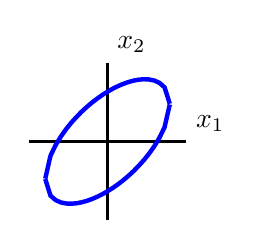
\begin{tikzpicture}[scale=0.5]
\draw[-, thick](-2,0)--(2,0);
\node[above right] at (2,0){$x_1$};
\draw[-, thick](0,-2)--(0,2);
\node[above right] at (0,2){$x_2$};
\draw[blue, ultra thick, domain=-1.58113:1.58113] plot(\x, {0.2*(3*\x-2*sqrt(2)*sqrt(5-2*\x*\x))});
\draw[blue, ultra thick, domain=-1.58113:1.58113] plot(\x, {0.2*(2*sqrt(2)*sqrt(5-2*\x*\x)+3*\x)});
\end{tikzpicture}
\end{center}

Use a change of variables to choose new axes such that the ellipse is oriented parallel to the new coordinate axes. In other words, use a change of variables to rewrite $q$ to eliminate the $x_1x_2$ term. 
\end{example}

\begin{solution}
First, express the level curve as $\vect{x}^TA\vect{x}$ where $\vect{x} = \leftB
\begin{array}{r}
x_1 \\
x_2 
\end{array}
\rightB$ and $A$ is symmetric. Let $A = \leftB \begin{array}{rr}
a_{11} & a_{12} \\
a_{21} & a_{22}
\end{array} \rightB$. Then $q = \vect{x}^T A \vect{x}$ is given by 
\begin{eqnarray*}
q &=&  \leftB \begin{array}{cc}
x_1 & x_2 
\end{array}
\rightB
\leftB \begin{array}{rr}
a_{11} & a_{12} \\
a_{21} & a_{22}
\end{array} \rightB
\leftB
\begin{array}{r}
x_1 \\
x_2 
\end{array}
\rightB\\
&=& a_{11}x_1^2 + (a_{12} + a_{21})x_1x_2 + a_{22}x_2^2
\end{eqnarray*}
 
Equating this to the given description for $q$, we have 
\[
5x_1^2 -6x_1x_2 + 5x_2^2 =  a_{11}x_1^2 + (a_{12} + a_{21})x_1x_2 + a_{22}x_2^2
\]
This implies that $a_{11} = 5, a_{22} = 5$ and in order for $A$ to be symmetric, $a_{12} = a_{22} = \frac{1}{2} (a_{12}+a_{21}) = -3$. The result is $A = \leftB
\begin{array}{rr}
5 & -3 \\
-3 & 5
\end{array}
\rightB$. We can write $q = \vect{x}^TA\vect{x}$ as 
\begin{equation*}
\leftB
\begin{array}{cc}
x_1 & x_2 
\end{array}
\rightB \leftB
\begin{array}{rr}
5 & -3 \\
-3 & 5
\end{array}
\rightB \leftB
\begin{array}{c}
x_1 \\
x_2
\end{array}
\rightB =8
\end{equation*}

Next, orthogonally diagonalize the matrix $A$ to write $U^TAU = D$. The details are left to the reader and the necessary matrices are given by 
\begin{eqnarray*}
U &=& \leftB \begin{array}{rr}
\vspace{0.05in}\frac{1}{2}\sqrt{2} & \vspace{0.05in}\frac{1}{2}\sqrt{2} \\
\vspace{0.05in}\frac{1}{2}\sqrt{2} & -\vspace{0.05in}\frac{1}{2}\sqrt{2}
\end{array}
\rightB \\
D &=& 
\leftB \begin{array}{rr}
2 & 0 \\
0 & 8 
\end{array}
\rightB
\end{eqnarray*}

Write $\vect{y} = \leftB \begin{array}{r}
y_1 \\
y_2 
\end{array} \rightB$, such that $\vect{x} = U \vect{y}$. Then it follows that $q$ is given by 
\begin{eqnarray*}
q &=& d_{11}y_1^2 + d_{22}y_2^2 \\
&=& 2y_1^{2}+8y_2^{2}
\end{eqnarray*}
Therefore the level curve can be written as $2y_1^{2}+8y_2^{2}=8$. 

This is an ellipse which is parallel to the coordinate axes. Its graph is of
the form

\begin{center}
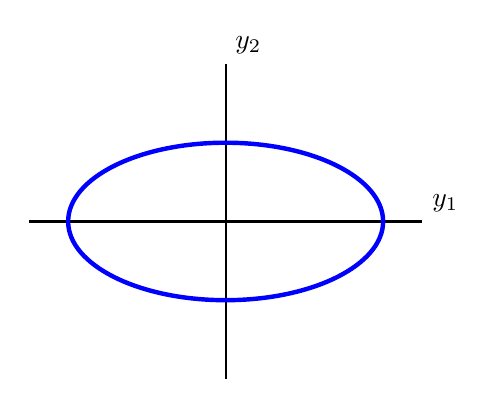
\begin{tikzpicture}
\draw[-, thick](-2.5,0)--(2.5,0);
\node[above right] at (2.5,0){$y_1$};
\draw[-, thick](0,-2)--(0,2);
\node[above right] at (0,2){$y_2$};
\draw[ultra thick, blue] (0,0) ellipse (2cm and 1cm);
\end{tikzpicture}
\end{center}

\noindent Thus this change of variables chooses new axes  such that with respect to these new axes, the
ellipse is oriented parallel to the coordinate axes.
\end{solution}